\documentclass[11pt,letterpaper]{article}
\usepackage[margin=0.60in,top=0.58in,bottom=0.56in]{geometry}
\usepackage{mathptmx}
\usepackage{microtype}
\usepackage{graphicx}
\usepackage{booktabs}
\usepackage{array}
\usepackage{longtable}
\usepackage{amsmath,amssymb}
\usepackage[hidelinks]{hyperref}
\setlength{\parindent}{0pt}
\setlength{\parskip}{2.5pt}
\setlength{\columnsep}{0.25in}
\setcounter{secnumdepth}{0}
\renewcommand{\section}[1]{\vspace{3pt}\noindent\textbf{\underline{#1}}\par\vspace{1pt}}
\renewcommand{\subsection}[1]{\vspace{2pt}\noindent\textbf{#1}\par\vspace{1pt}}
\renewcommand{\familydefault}{\rmdefault}
\providecommand{\tightlist}{\setlength{\itemsep}{0pt}\setlength{\parskip}{0pt}}
\providecommand{\pandocbounded}[1]{\sbox0{#1}\ifdim\wd0>\linewidth\resizebox{\linewidth}{!}{#1}\else\usebox0\fi}
\title{\vspace{-1.2em}\textbf{\MakeUppercase{Neurologically Motivated
Self-Supervised Learning for Bilateral Gait Geometry}}\vspace{-0.5em}}
\author{\normalsize [Authors and affiliations to be inserted in the RISEx template]}
\date{}
\begin{document}
\twocolumn[
  \begin{@twocolumnfalse}
  \maketitle
  \vspace{-1.1em}
  \end{@twocolumnfalse}
]
\subsection{INTRODUCTION}\label{introduction}

Learning from videos of people could help robots anticipate human
motion, but an internal feature match is an incomplete test of what a
representation preserves. We evaluate a skeleton JEPA with a geometric
relation that has a known answer. Reflection swaps left and right
anatomy and reverses a signed speed difference. Gait asymmetry has been
studied in stroke, Parkinson's disease, cerebral palsy, and muscular
disorders {[}1--3{]}. Those studies motivate the relation; this work
neither diagnoses these conditions nor estimates disease severity.

\subsection{MATERIALS AND METHODS}\label{materials-and-methods}

We selected 625 pose sequences from 93 GAVD source videos {[}4{]}.
Processing is clip-local. It retains all 33 landmarks in a 64-by-33-by-3
array, then packs four frames per token to preserve a 16-by-33
spatial-temporal grid. The online encoder receives visible tokens, while
a predictor estimates hidden teacher features. The teacher follows the
online encoder by exponential moving average. This pretraining uses no
movement target or disease label.

The target averages normalized left-minus-right median speed differences
for five anatomical pairs. A frozen ridge readout is fitted only on
outer-training sources. Five outer source-video folds keep test clips,
transformed views, encoder training, and supervised readout fitting
separate. Five seeds share initialization, source draws, views, and
updates within each mask comparison. We report source-balanced scores
and paired source resampling that keeps all clips and seed predictions
from a source together.

\subsection{RESULTS AND DISCUSSION}\label{results-and-discussion}

\begin{figure}
\centering
\pandocbounded{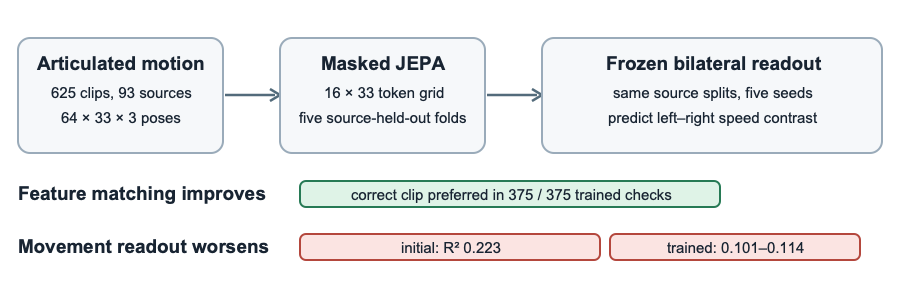
\includegraphics[keepaspectratio,alt={Study design and primary result: correctly matched latent features improve while the bilateral movement readout declines.}]{risex_onepage_evidence.png}}
\caption{Study design and primary result: correctly matched latent
features improve while the bilateral movement readout declines.}
\end{figure}

The initial encoder achieved \(R^2=0.223\). Trained teachers achieved
\(0.101\)--\(0.114\); every training arm was lower than its matched
initialization (difference \(-0.109\) to \(-0.122\)). Conversely,
correct-clip targets had lower feature error in 375/375 trained
diagnostic checks, versus 33/75 at initialization. Alternative motion
and connected-region masks gave intervals spanning zero relative to
matched random masks.

The result is a controlled warning for learned articulated-motion
features. It remains conditional on the target and readout: preparation
changes the score, and the larger readout combines motion, dimension,
and missingness changes. It therefore cannot establish a general loss of
geometric information or a robotics failure.

\subsection{CONCLUSIONS}\label{conclusions}

Latent feature correspondence and recovery of bilateral movement can
disagree. A geometric observable, matched initialization, and
source-held-out test split provide a compact evaluation pattern for AI
representations of articulated motion.

\subsection{REFERENCES}\label{references}

{[}1{]} Patterson KK et al.~\emph{Arch Phys Med Rehabil} 89:304--310,
2008. {[}2{]} Lewek MD et al.~\emph{Gait Posture} 31:256--260, 2010.
{[}3{]} Brændvik SM et al.~\emph{Front Neurol} 10:1399, 2020. {[}4{]}
Ranjan R et al.~\emph{IEEE Access} 13:45321--45339, 2025.
\end{document}
